\chapter{RISC-V}

\section{ABI e Istruzioni}
Il RISC-V si compone di 32 registri general purpose (x0-x31) di lunghezza differente a seconda della versione (RV32 o RV64). La \textbf{Application to Binary Interface} (ABI) è lo strumenti utilizzato per definire lo scopo di ciascun registro, assegnando a ognuno di questi un alias [\ref{fig:abi}]. Una tale suddivisione standardizzata aiuta il programmatore a scrivere codice più leggibile e strutturato: sapendo quali registri usare per specifiche funzioni, il codice risulta più prevedibile e manutenibile. 
\begin{figure}[!h]
	\centering
	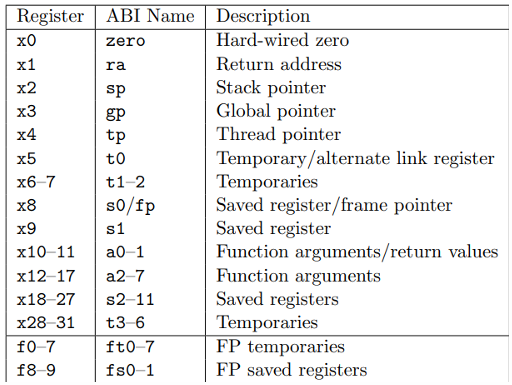
\includegraphics[width=0.5\linewidth]{img/abi}
	\caption{Nome ABI di alcuni dei registri più importanti.}
	\label{fig:abi}
\end{figure}
Il registro x0 è di sola lettura e contiene sempre valore zero, ed è utile nelle istruzioni che necessitano di un valore zero senza utilizzare un immediato. Il \textbf{formato delle istruzioni} è basato su lunghezza fissa pari a 32 bit (anche per la versione RV64). In particolare, il RISC-V possiede soltanto 47 istruzioni, tutto ciò che non rientra in queste viene gestito con delle estensioni ISA. Ciascuna istruzione può appartenere a uno dei seguenti tipi:
\begin{itemize}
	\item \textbf{R (Register)}: A questa categoria appartengono le istruzioni aritmetiche su registri. Nell'istruzione vengono inclusi gli operandi (registri) sorgente e destinazione.
	\item \textbf{I (Immediate and Load)}: A questa categoria appartengono le istruzioni aritmetiche con immediati e di load. Nell'istruzione vengono specificati gli operandi (registri) sorgente e destinazione, e l'immediato su 12 bit. Nel caso di \textit{load}, viene utilizzato un immediato come offset per accedere a un area di memoria.
	\item \textbf{S (Store)}: A questa categoria appartengono le istruzioni di \textit{store}, in cui la destinazione non è un registro ma una locazione di memoria (operando implicito).
	\item \textbf{U (Upper immediate)}: A questa categoria appartengono solo due istruzioni, che richiedono uno spazio maggiore per codificare un immediato di grandi dimensioni. Queste sono \textit{load upper immediate} (lui) e \textit{add upper immediate to program counter} (auipc).
	\item \textbf{J (Jump)}: A questa categoria appartengono le istruzioni di salto incondizionato con un offset con segno. Le due istruzioni possibili sono \textit{jump and link} (jal) e \textit{jump and link register} (jalr).
	\item \textbf{B (Branch)}: A questa categoria appartengono le istruzioni di salto condizionato. In particolare, l'offset utilizzabile viene codificato su 12 bit, per cui il salto è limitato a \(\pm2^{12}\) half-words (2 bytes), ovvero un range di \(\pm\)4 KiB. Il salto avviene se la condizione da verificare assume valore true.
\end{itemize}
A seconda del tipo, la struttura di ciascuna istruzione cambia, ovvero varia il modo in cui i 32 bit nella stringa vengono interpretati. L'unica cosa che resta invariata sono i bit relativi al campo \textit{opcode}, che vanno da 0 a 6. Notiamo come in alcune istruzioni sia presente un campo \textit{function} oltre a quello di opcode, il motivo di una tale scelta è semplificare la decodifica delle istruzioni. L'opcode individua una generica categoria di istruzioni (ad esempio, operazioni aritmetiche), mentre function specifica l'operazione esatta da eseguire (add, multiply, eccetera).
Gli operandi sono inclusi nelle istruzioni. L'architettura RISC-V appartiene chiaramente alla categoria di \textit{load and store} (essendo RISC), per cui non sono ammesse operazioni direttamente in memoria e non servono altre istruzioni per caricare gli operandi.

\subsection{Jump and Link e Jump and Link Register}
L'istruzione \textbf{jal} permette di effettuare salti incondizionati con un offset con segno. L'offset viene codificato come un immediato su 21 bit, per cui il range del salto è limitato a \(\pm2^{20}\) half-words (2 bytes), ovvero \(\pm\) 1 MiB. Può essere utile per implementare statement di tipo \textit{goto} o chiamate a funzioni.
\[pc=pc+signed(imm[20:0])\]
\\
\\
L'istruzione \textbf{jalr} permette anch'essa salti incondizionati con offset con segno, questa volta non incrementando il PC con l'offset, ma sommando l'offset a una locazione di memoria conservata in un registro. Questo permette dei salti di dimensione pari a \(\pm2^{32}\), ovvero \(\pm\) 4 GiB. Risulta utile per implementare ritorni da chiamate a funzioni.
\[pc=rs1+signed(imm[11:0])\]

\subsection{Cheatsheet}
Riportiamo un \textbf{cheatsheet} contenente le principali istruzioni, utili a implementare programmi di base, delle 47 disponibili nell'ISA base del RISC-V (RV32I).
\begin{itemize}
	\item Aritmetica (tipo R e I)
	\begin{itemize}
		\item \textit{add rd, rs1, rs2 → rd = rs1 + rs2}
		\item \textit{addi rd, rs1, imm → rd = rs1 + imm}
		\item \textit{sub rd, rs1, rs2 → rd = rs1 - rs2}
		\item \textit{and rd, rs1, rs2 → rd = rs1 \& rs2} (anche com immediato)
		\item \textit{or rd, rs1, rs2 → rd = rs1 | rs2} (anche com immediato)
	\end{itemize}
	\item Confronti
	\begin{itemize}
		\item \textit{slt rd, rs1, rs2} → setta \textit{rd} a 1 se \textit{rs1 < rs2}, altrimenti a 0
		\item \textit{slti rd, rs1, imm} → setta \textit{rd} a 1 se \textit{rs1 < imm}, altrimenti a 0		
	\end{itemize}
	\item Accesso alla memoria (load/store)
	\begin{itemize}
		\item \textit{lw rd, offset(rs1)} → load della word dalla locazione \textit{(rs1 + offset)} in \textit{rd}
		\item \textit{lh rd, offset(rs1)} → load della half-word dalla locazione \textit{(rs1 + offset)} in \textit{rd}
		\item \textit{lb rd, offset(rs1)} → load del byte dalla locazione \textit{(rs1 + offset)} in \textit{rd}
		\item \textit{sw rs2, offset(rs1)} → store della word \textit{rs2} nella locazione \textit{(rs1 + offset) }
		\item \textit{sh rs2, offset(rs1)} → store della half-word \textit{rs2} nella locazione \textit{(rs1 + offset) }
		\item \textit{sb rs2, offset(rs1)} → store del byte \textit{rs2} nella locazione \textit{(rs1 + offset) }
	\end{itemize}
	\item Salti condizionati (branch)
	\begin{itemize}
		\item \textit{beq rs1, rs2, label} → salta a \textit{label} se \textit{rs1 = rs2}
		\item \textit{bne rs1, rs2, label} → salta a \textit{label} se \textit{rs1 != rs2}
		\item \textit{blt rs1, rs2, label} → salta a \textit{label} se \textit{rs1 < rs2} 
		\item \textit{bge rs1, rs2, label} → salta a \textit{label} se \textit{rs1 >= rs2}
	\end{itemize}
	\item Salti e chiamate
	\begin{itemize}
		\item \textit{jal rd, offset} → salta all'indirizzo \textit{PC + offset} e salva l'indirizzo di ritorno in \textit{rd} (solitamente \textit{ra dell'ABI})
		\item \textit{jalr rd, rs1, offset} → salta all'indirizzo \textit{(rs1 + offset) \& ~1} e salva l'indirizzo di ritorno in \textit{rd} (solitamente \textit{ra} dell'ABI)
		\item \textit{ecall} → chiamata a sistema (system call)
	\end{itemize}
\end{itemize}
Riportiamo l'esercizio proposto a lezione, che richiede di copiare un vettore in memoria in un altro. Si nota l'uso della pseudo-istruzione \textit{la} (load address), messa a disposizione dal compilatore per caricare un indirizzo. Si rimanda al paragrafo delle pseudo-istruzioni per ulteriori dettagli [\ref{{subsec:pseudo}}].
\begin{lstlisting}
main:
    la   a0, src       # carica indirizzo sorgente in a0
	la   a1, dst       # carica indirizzo destinazione in a1
    la   t0, len       # carica indirizzo di len in t0
	lw   a2, 0(t0)     # carica valore di len in a2
	jal  ra, copia     # chiama funzione copia, salva ritorno in ra	
	
copia:								# funzione per copiare
	beq  a2, x0, fine   # se lenght == 0, termina
ciclo:
	lw   t0, 0(a0)      # carica elemento da src
	sw   t0, 0(a1)      # scrive elemento in dst
	addi a0, a0, 4      # src ++
	addi a1, a1, 4      # dst ++
	addi a2, a2, -1     # length --
	bne  a2, x0, ciclo  # se length != 0 ripeti	
fine:
	jalr x0, ra, 0      # ritorna al chiamante (main)
\end{lstlisting}

\section{Livelli di privilegio e Interruzioni}
Il RISC-V supporta tre \textbf{livelli di privilegio}: \textit{User}, \textit{Supervisor} e \textit{Machine} [\ref{fig:risc-v-privilege}].
\begin{figure}[!h]
	\centering
	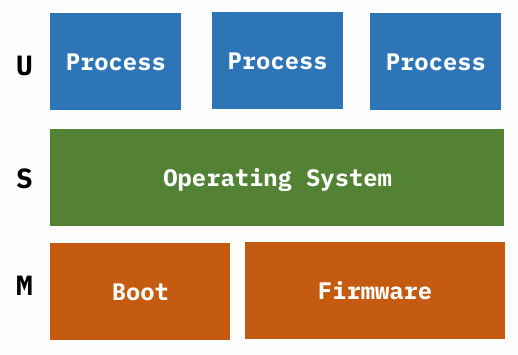
\includegraphics[width=0.3\linewidth]{img/risc-v-privilege}
	\caption{Livelli di privilegio del RISC-V.}
	\label{fig:risc-v-privilege}
\end{figure}
Un insieme di registri, noto come \textbf{Control and Status Registers} (CSRs), ha il compito di rappresentare lo stato dell'architettura (stato della CPU, interruzioni, eccezioni, eccetera). Questi sono localizzati in uno spazio di indirizzamento privato e possono essere acceduti solo tramite istruzioni speciali:
\begin{itemize}
	\item Istruzioni di \textit{read} e \textit{write}.
	\item Istruzioni di \textit{set} e \textit{clear}.
	\item Varianti delle istruzioni con registri e immediati.
\end{itemize}

Per quanto riguarda la \textbf{gestione delle interruzioni ed eccezioni}, questa avviene tramite i CSRs in due fasi:
\begin{itemize}
	\item \textbf{Fase offline}: Avviene durante il boot del sistema e viene eseguito del codice speciale che: 
	\begin{enumerate}
		\item Abilita un bit speciale per le interruzioni. In particolare, il bit \textit{MIE} nel CSR \textit{mstatus}, che si occupa dello stato della CPU.
		\item Abilita tutti gli specifici interrupt interessati tramite i bit di un secondo registro. In altre parole, si smascherano i bit del CSR \textit{mie} corrispondenti alle linee di interruzione che interessano.
	\end{enumerate}
	\item \textbf{Fase online}: Accade quando effettivamente si verifica un'interruzione o un’eccezione.
	\begin{enumerate}
		\item La CPU salva il PC in un apposito registro, il \textit{mepc}.
		\item La CPU salta all’indirizzo nel registro \textit{mtvec}, il quale contiene l’indirizzo della tabella dei vettori.
		\item La CPU salta al gestore dell’interrupt (handler). Il modo in cui viene prelevato l'indirizzo dipende da se le interruzioni sono vettorizzate, specificato nel registro \textit{mcause}.
		\item Il gestore termina con l’istruzione \textit{mret}, che permette di ritornare dal trap 
		ripristinando il valore del PC da \textit{mepc}.
	\end{enumerate}
\end{itemize}
RISC-V introduce delle istruzioni privilegiate chiamate \textbf{system instructions}, usate da sistemi operativi e ambienti virtualizzati per gestire system calls e sincronizzazione. Possono inoltre essere utilizzate per il debugging, ma richiedono un modulo esterno per funzionare.
\\
\\
Il \textbf{Supervisor Binary Interface} (SBI) è un'interfaccia standard per permettere al software a livello supervisor (S-mode) di funzionare su hardware diversi, mantenendolo portabile. OpenSBI è la piattaforma open-source più usata per implementare SBI.

\section{Estensioni}
Una delle più importanti \textbf{estensioni} del RISC-V è \textit{RV64}, nella quale registri e CSRs hanno una dimensione di 64 bit, anche se le istruzioni sono sempre di lunghezza pari a 32 bit. Sono incluse delle specifiche istruzioni per manipolare dati a 32 bit, utili per compatibilità o efficienza.
\\
\\
Il nucleo base di RISC-V (RV32I) ha solo 47 istruzioni, per cui è molto semplice e minimale. Per questo motivo, l'architettura è estendibile e modulare, in modo da adattarla alle esigenze del sistema. Si può estendere aggiungendo nuove funzionalità tramite \textbf{estensioni}, ciascuna con un proprio \textit{opcode}. Le implementazioni RISC-V vengono identificate dal nome delle estensioni supportate, ad esempio: RV32IA = RV32I (base) + A (Atomic Instructions).
\\
\\
Un possibile esempio è RV32E, una variante semplificata di RV32I pensata per microcontrollori o sistemi con pochissime risorse. Riduce i registri da 32 a solo 16, occupando meno spazio sull’hardware. L'estensione di tipo C, invece, utilizza istruzioni compresse da 16 bit (anziché 32), permettendo di ridurre la dimensione del codice in memoria.

\section{Pseudo-istruzioni}
\label{subsec:pseudo}
Le \textbf{pseudo-istruzioni} sono delle scorciatoie per il programmatore che permettono di scrivere codice più leggibile e facile da scrivere, ma che non appartengono all'ABI. In altre parole, non esiste una corrispondenza con il codice macchina, è compito dell'assemblatore convertirle in istruzioni comprensibili all'hardware.
\\
\\
Supponiamo ad esempio di voler fare la \textit{load} di un immediato molto grande, più dei 12 bit normalmente disponibili, in un registro. Usando la pseudo-istruzione \textit{li} è possibile scaricare questo compito complesso all'assemblatore, che scomporrà la \textit{load} in tante \textit{load} e \textit{add} diverse, incrementando il valore con diverse operazioni.

\section{Calling convention}
La \textbf{Calling Convention} definisce le regole che governano come le funzioni si chiamano tra loro e gestiscono parametri e valori di ritorno. Tipicamente, il processo avviene attraverso alcune fase alternate tra chiamante e funzione chiamata:
\begin{itemize}
	\item Caller (chi chiama):
	\begin{enumerate}
		\item Salva il proprio contesto sullo stack, includendo i registri.
		\item Salva l'indirizzo di ritorno in a0-a7 e se necessario pusha eventuali parametri sullo stack.
		\item Utilizza l'istruzione \textit{jal} per saltare alla procedura, salvando l'indirizzo di ritorno in \textit{ra}.
	\end{enumerate}
	\item Callee (funzione chiamata):
	\begin{enumerate}
		\item Preleva gli eventuali parametri dallo stack.
		\item Effettua le operazioni.
		\item Memorizza il risultato da ritornare in a0-a1.
		\item Utilizza la pseudo-istruzione \textit{ret} per ritornare al chiamante.
	\end{enumerate}
	\item Caller (chi chiama):
		\begin{enumerate}
		\item Ripristina il contesto salvato precedentemente sullo stack.
		\item Legge il valore ritornato da a0-a1.
	\end{enumerate}
\end{itemize}

\subsection{Stack}
La convenzione adottata dal RISC-V è che lo \textbf{stack} cresca dall'alto verso il basso in termini di indirizzi. Per gestire lo stack frame sono presenti due CSRs:
\begin{itemize}
	\item \textbf{Stack Pointer (sp)}: Punta alla base del corrente stack frame.
	\item \textbf{Frame Pointer (fp)}: (Normalmente) punta alla fine del precedente stack frame. Normalmente non viene utilizzato, in quanto non è obbligatorio dell'implementazione del RISC-V. Tuttavia esistono diversi vantaggi nel suo impiego, ad esempio l'indirizzo di ritorno ha un offset fissato dal \textit{fp} corrente.
\end{itemize}
Ricordiamo che lo stack frame è una porzione di memoria nello stack che viene allocata ogni volta che una funzione viene chiamata [\ref{fig:stack-frame}]. Serve a gestire le variabili locali, parametri, indirizzo di ritorno, e registri salvati.
\begin{figure}[!h]
	\centering
	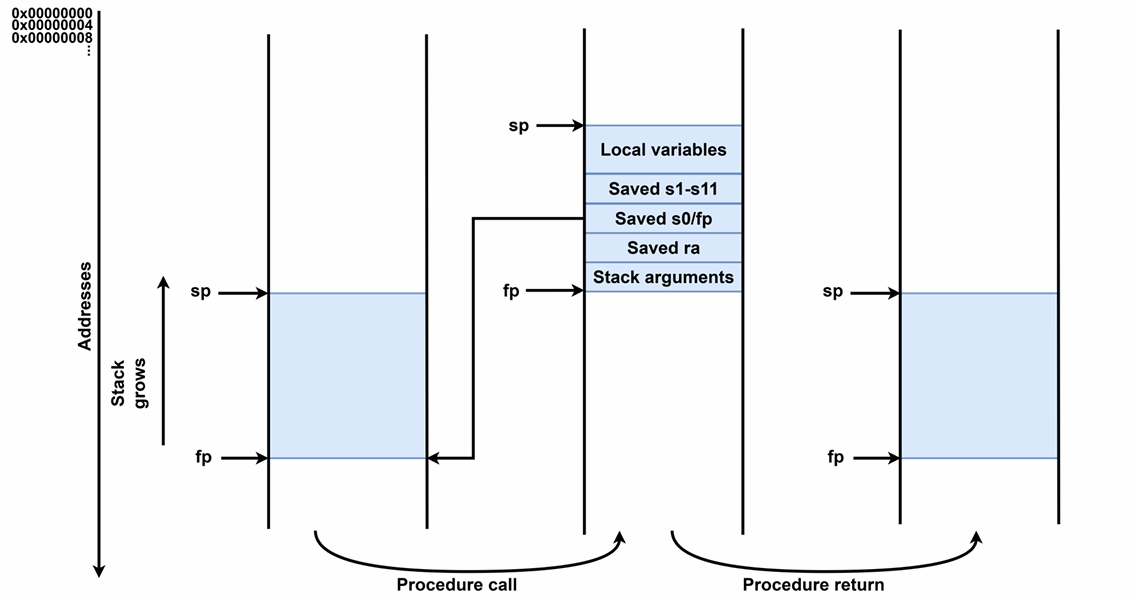
\includegraphics[width=0.6\linewidth]{img/stack-frame}
	\caption{Esempio di stack frame nel RISC-V.}
	\label{fig:stack-frame}
\end{figure}
\MakeUppercase{è} fondamentale notare che l'uso esatto del registro \textit{fp} non è fisso e può cambiare in base al compilatore usato e alle opzioni di compilazione. Nel RISC-V, il frame pointer è solitamente s0, ma non obbligatoriamente.

\section{Confronto con il MIPS}
L'ISA del MIPS presenta molte similitudini con quella del RISC-V, poiché entrambe seguono una stessa filosofia di design.
\begin{itemize}
	\item \textbf{Istruzioni}: Entrambe hanno istruzioni a lunghezza fissa di 32 bit.
	\item \textbf{Registri}: Entrambe hanno 32 registri general purpose.
	\item \textbf{Supporto 64-bit}: Entrambe supportano versioni a 64 bit (RV64 e MIPS-64).
	\item \textbf{Architettura}: Entrambe sono di tipo load and store.
	\item \textbf{Salti condizionati}: Mentre il RISC-V offre diverse modalità di comparazione (beq, bne, blt, bge, eccetera), il MIS ne possiede solo due (beq e bne).
\end{itemize}
Inoltre, i mnemonici delle istruzioni sono perlopiù identici, tranne qualche piccola eccezione.
\\
\\
Si consiglia una lettura del documento "Domande RISC-V" presente sul team, in quanto ci sono molte domande (con le rispettive risposte) \textit{particolari} per comprendere meglio alcuni dettagli su questa architettura.